\section{Results}

Examples of results of antipatterns and patterns found in two of our APIs Twitter and GitHub are illustrated below in Figures \ref{fig:githubBarAntiEx}, \ref{fig:githubBarPattEx}, \ref{fig:twitterBarAntiEx}, and \ref{fig:twitterBarPattEx}. For the complete results on the detection of patterns and antipatterns for all analysed API endpoints, see Appendix 1. Each endpoint can contain multiple antipatterns or patterns. We performed the detection of eleven antipatterns and eight patterns.

\begin{figure}[htb!]
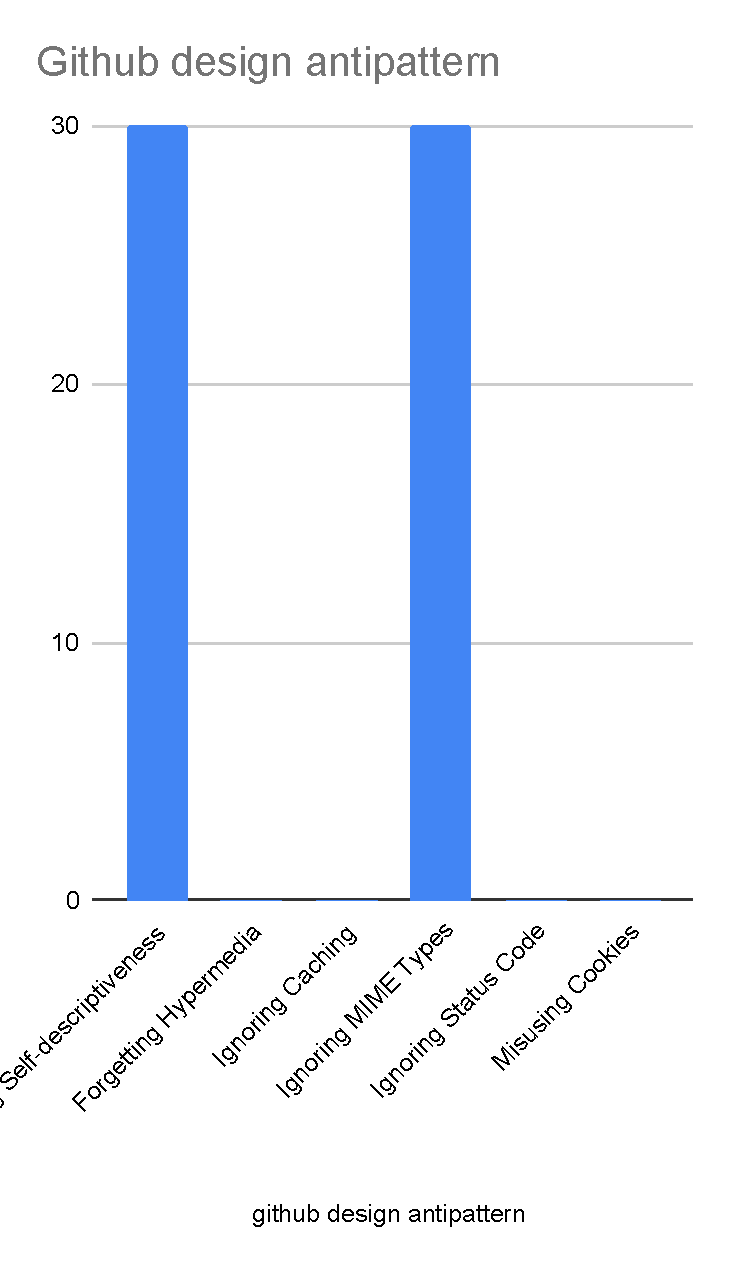
\includegraphics[width=0.5\textwidth]{img/exampleBars/githubAntiDes.pdf}
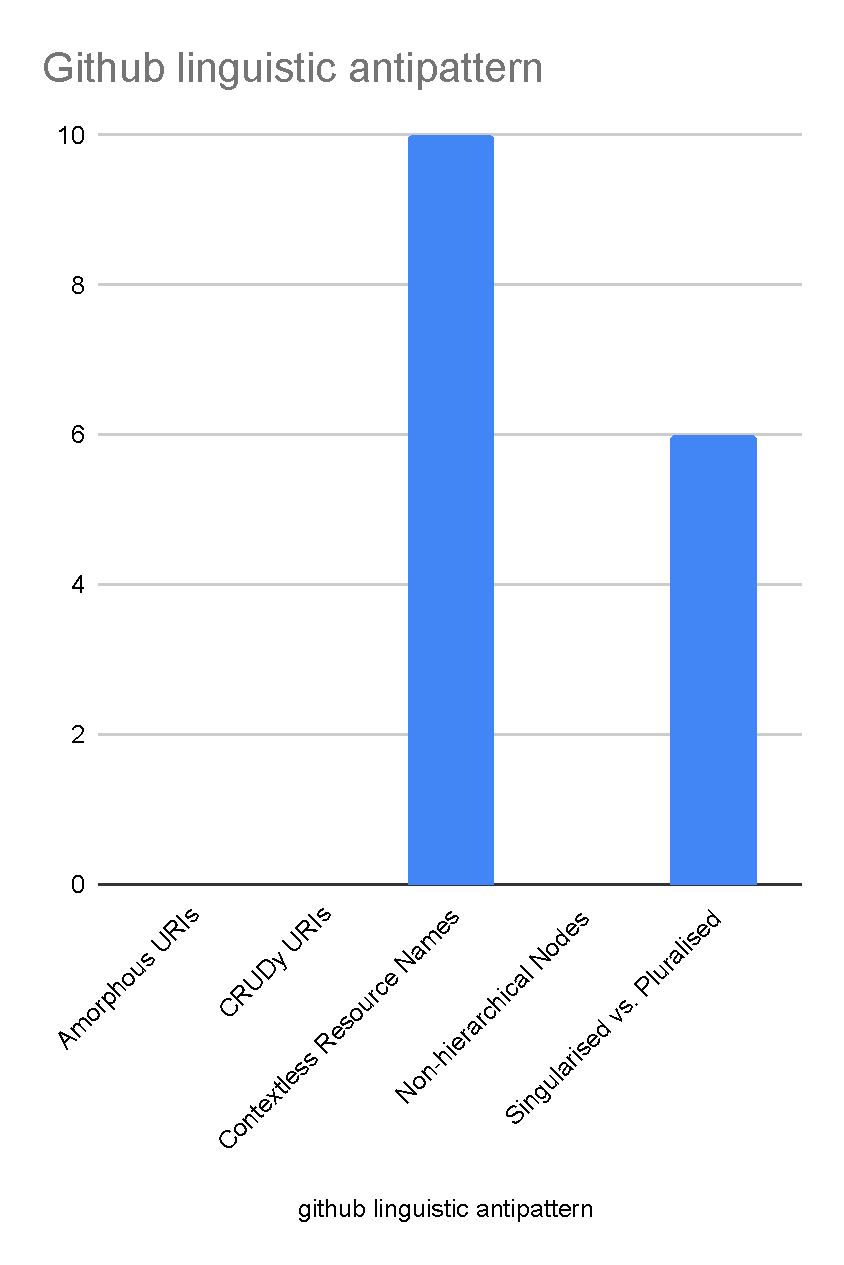
\includegraphics[width=0.5\textwidth]{img/exampleBars/githubAntiLing.pdf}
\caption{Github antipatterns.}
\label{fig:githubBarAntiEx}
\end{figure}

\begin{figure}[htb!]
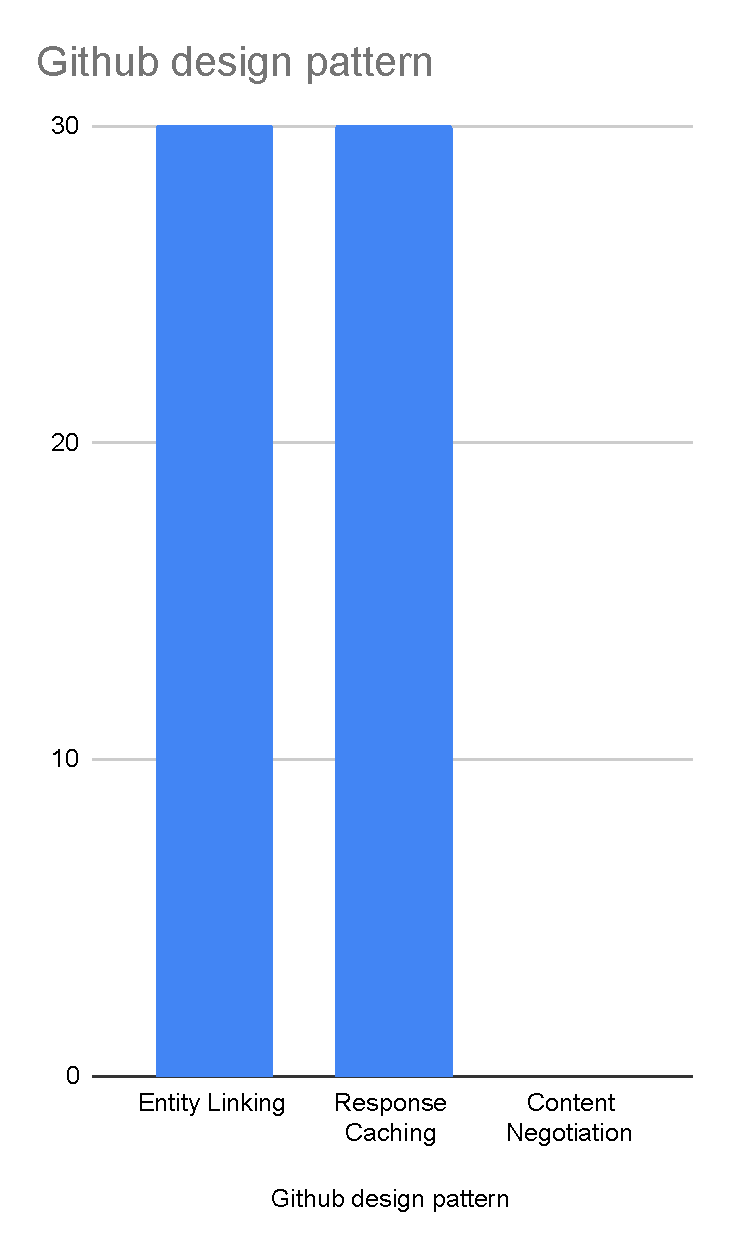
\includegraphics[width=0.5\textwidth]{img/exampleBars/githubDesPatt.pdf}
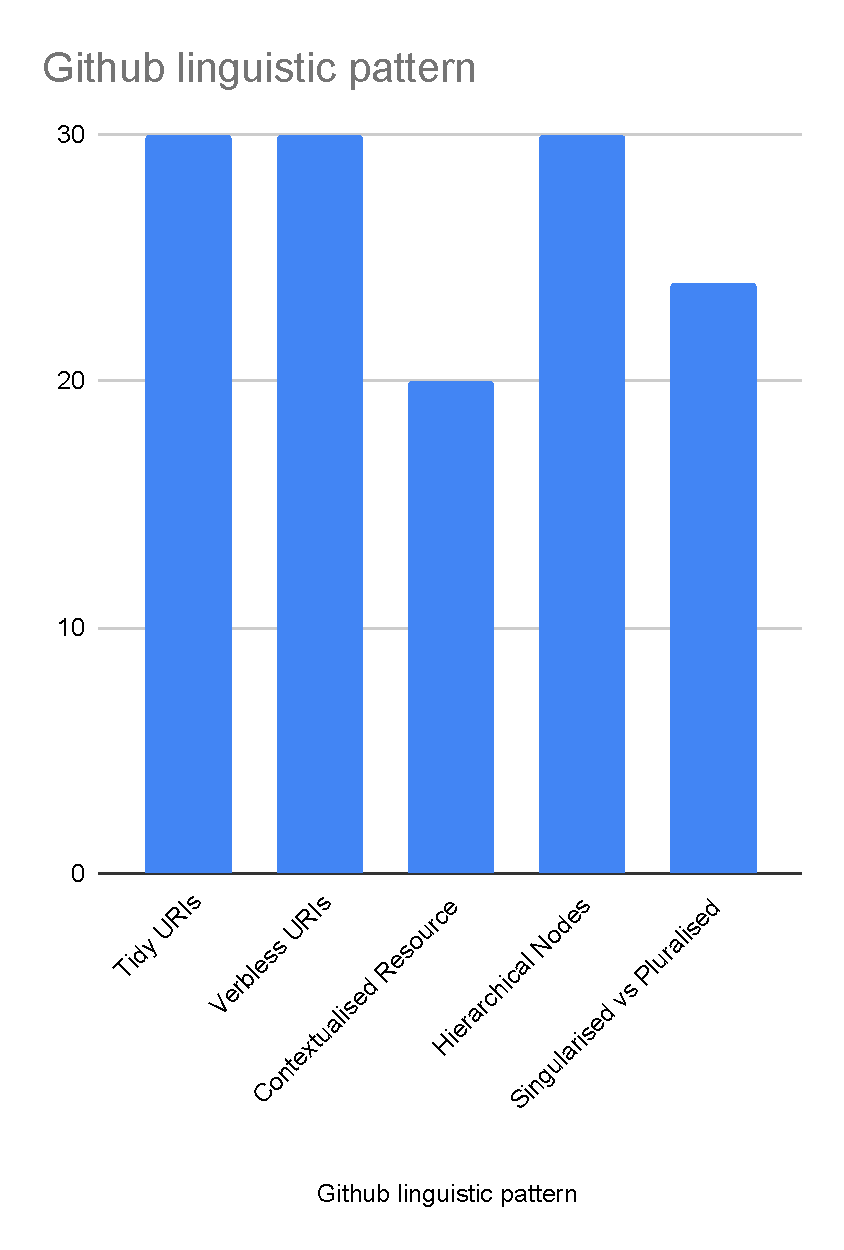
\includegraphics[width=0.5\textwidth]{img/exampleBars/githubLingPatt.pdf}
\caption{Github patterns.}
\label{fig:githubBarPattEx}
\end{figure}

\begin{figure}[htb!]
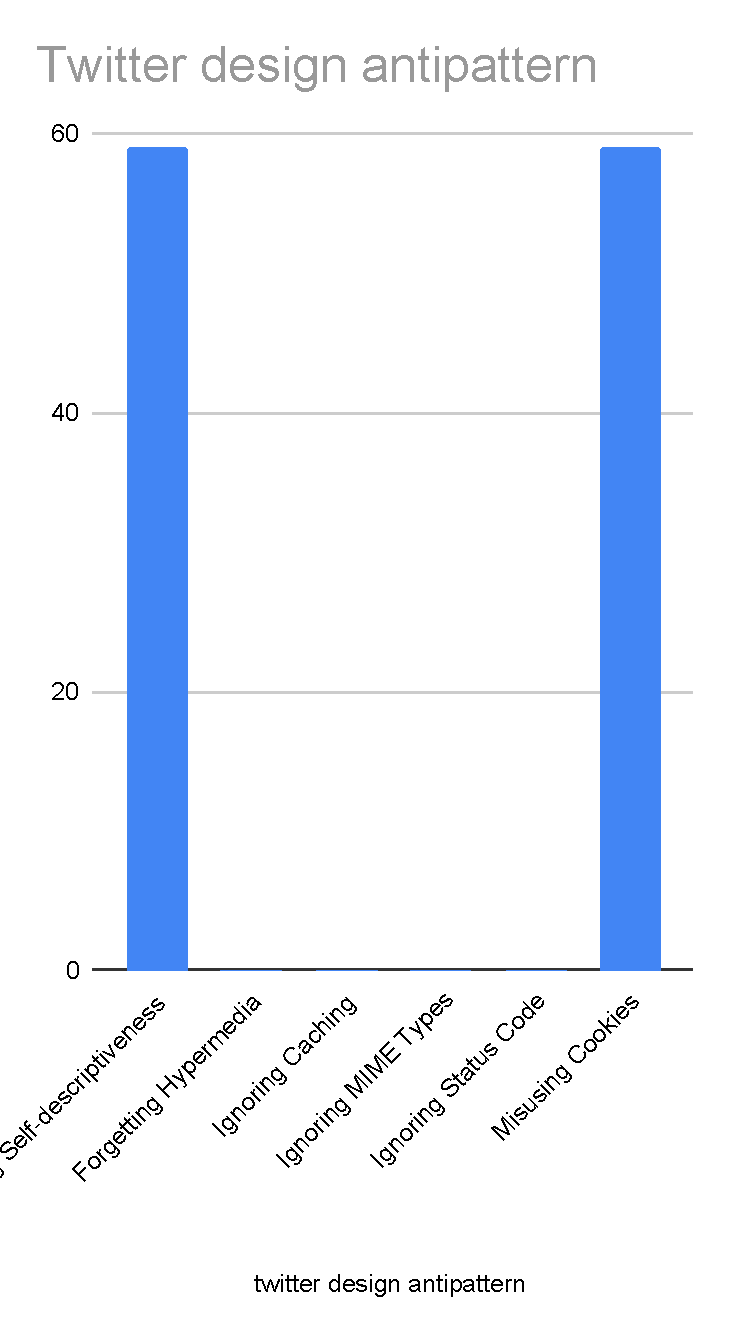
\includegraphics[width=0.5\textwidth]{img/exampleBars/twitterDesPatt.pdf}
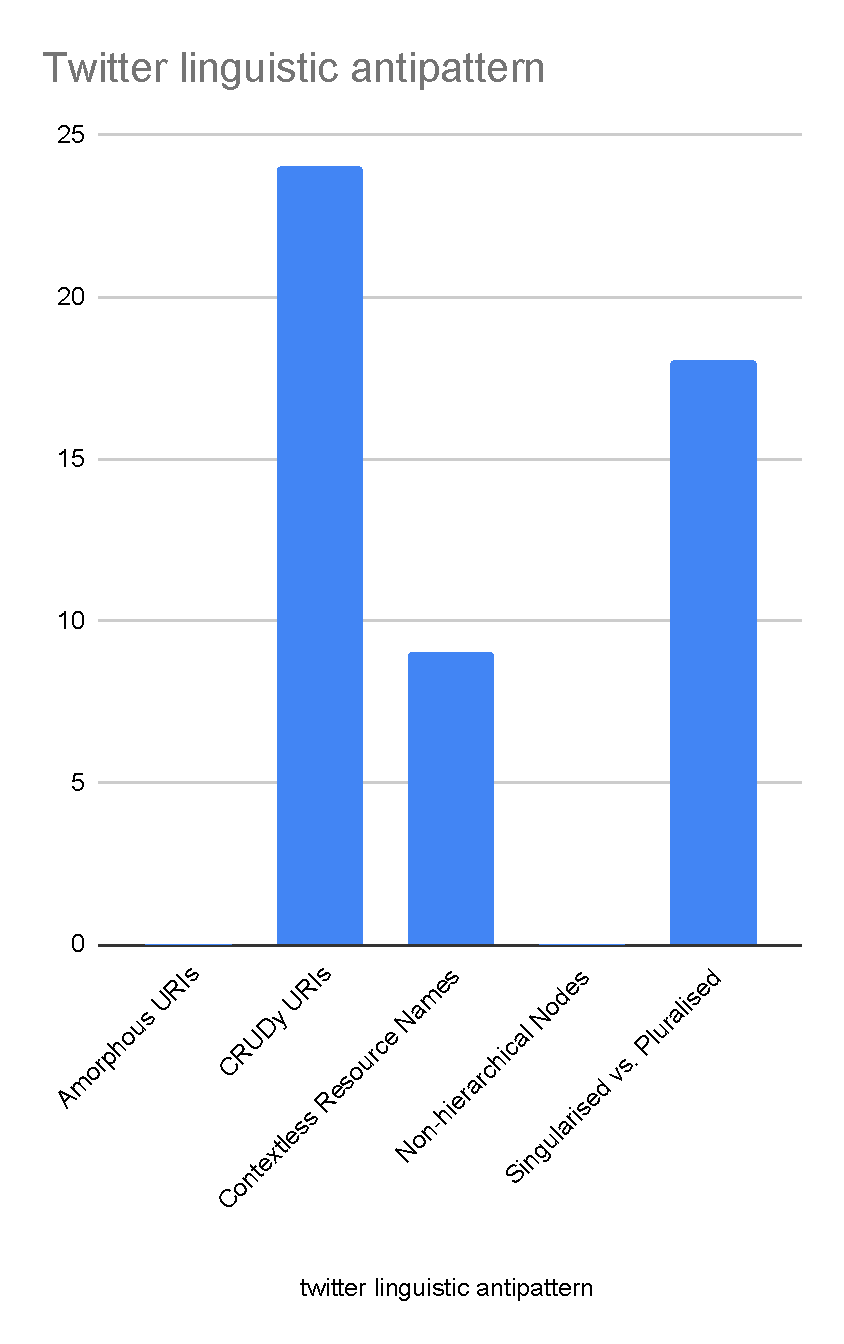
\includegraphics[width=0.5\textwidth]{img/exampleBars/twitterLingAnti.pdf}
\caption{Twitter antipatterns.}
\label{fig:twitterBarAntiEx}
\end{figure}

\begin{figure}[htb!]
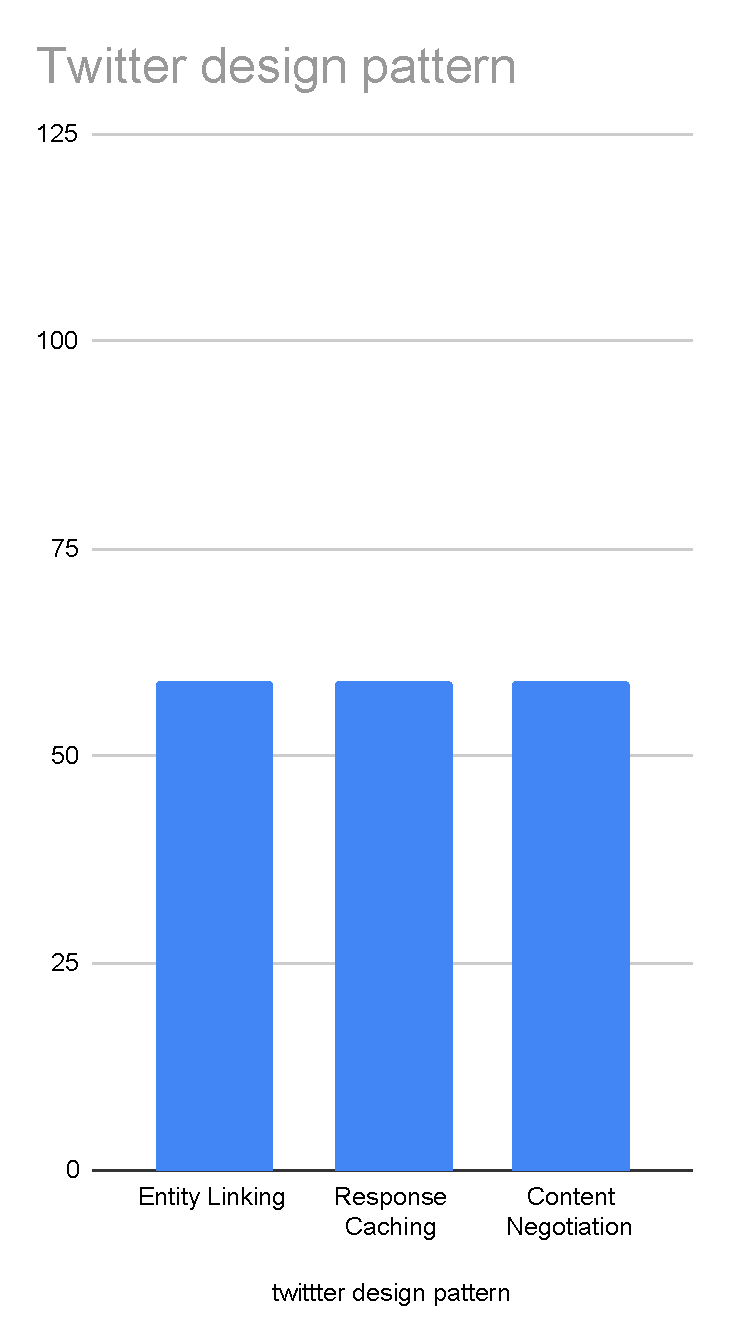
\includegraphics[width=0.5\textwidth]{img/exampleBars/twitterDesAnti.pdf}
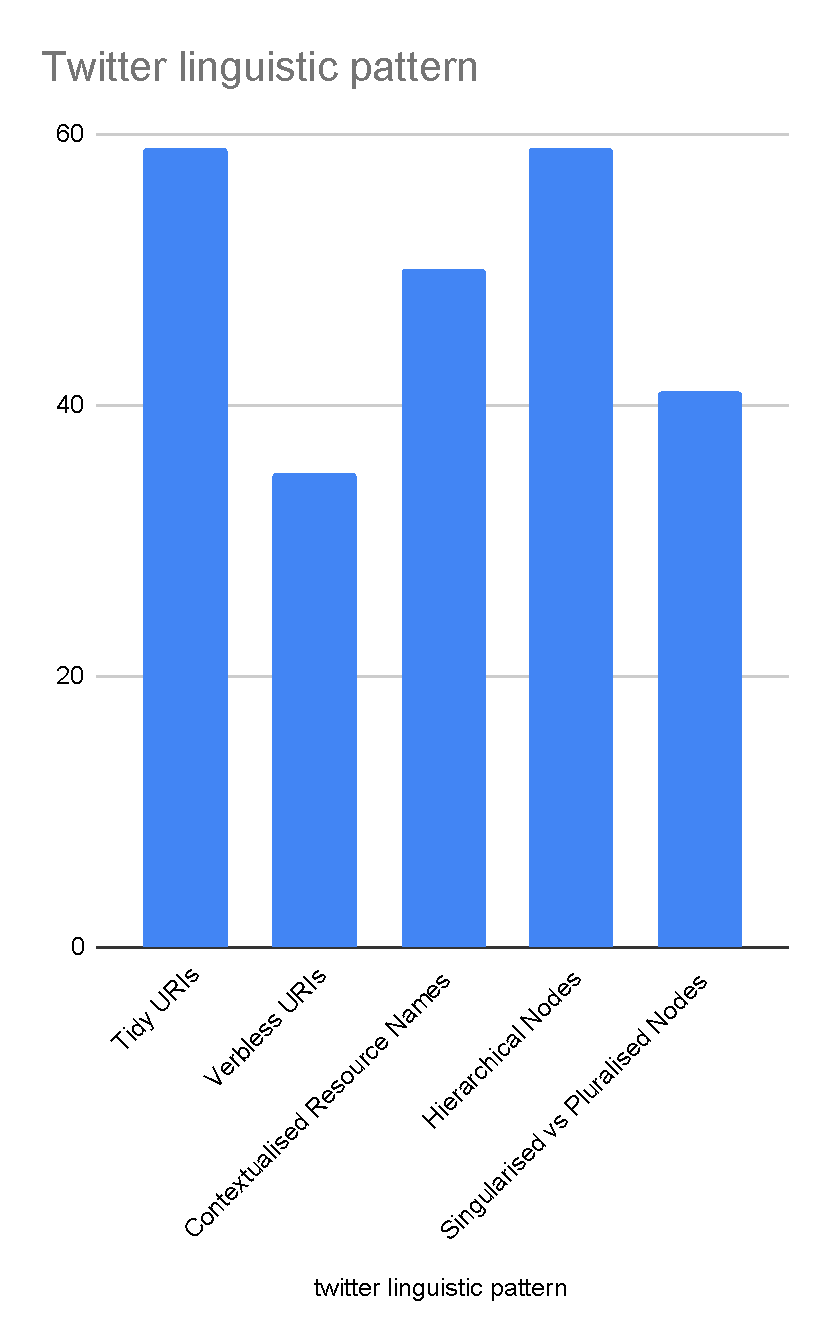
\includegraphics[width=0.5\textwidth]{img/exampleBars/twitterLingPatt.pdf}
\caption{Twitter patterns.}
\label{fig:twitterBarPattEx}
\end{figure}

\clearpage

\subsection{RQ1: Is there a relation between design and linguistic quality in RESTful APIs?}

\begin{table}[ht!]
\scriptsize
\setlength{\tabcolsep}{1.5pt}
\begin{tabular}{|p{18mm}|p{14mm}|p{9mm}|p{13mm}|p{11mm}|p{14mm}|p{7mm}|p{10mm}|p{17mm}|p{12mm}|p{14mm}|}
\hline Antipatterns & Amorphous URI & CRUDy URIs & Contextless Resource & Pluralised Nodes & Non-hierarchical Nodes & Tidy URIs & Verbless URIs & Contextualised Resource & Pluralised Nodes Pattern & Hierarchical Nodes  \\
\hline 
 Breaking Self-descriptiveness &
 36 &
 28 &
 53 &
 39 &
 0 &
 281 &
 289 &
 264 &
 278 &
 317
\\ \hline
 Forgetting Hypermedia &
 0 &
 0 &
 0 &
 0 &
 0 &
 0 &
 0 &
 0 &
 0 &
 0
\\ \hline
 Misusing Cookies &
 0 &
 24 &
 14 &
 21 &
 0 &
 100 &
 76 &
 86 &
 79 &
 100
\\ \hline
Ignoring MIME Types &
 0 &
 0 &
 12 &
 6 &
 0 &
 89 &
 89 &
 77 &
 83 &
 89
\\ \hline
Ignoring Status Code &
 0 &
 1 &
 4 &
 0 &
 0 &
 4 &
 3 &
 0 &
 4 &
 4
\\ \hline
Ignoring Caching &
 0 &
 0 &
 0 &
 0 &
 0 &
 0 &
 0 &
 0 &
 0 &
 0
\\ \hline
Entity linking &
 36 &
 28 &
 57 &
 39 &
 0 &
 290 &
 298 &
 269 &
 287 &
 326
\\ \hline
Content Negotiation &
 36 &
 28 &
 45 &
 33 &
 0 &
 201 &
 209 &
 192 &
 204 &
 237
\\ \hline
Response Caching &
 36 &
 28 &
 57 &
 39 &
 0 &
 290 &
 298 &
 269 &
 287 &
 326
\\ \hline
\end{tabular}
\caption{Contingency table on the set of design and linguistic patterns and antipatterns.}
\label{contingencytable}
\end{table}

Table \ref{contingencytable} shows the contingency table combining the design and linguistic patterns and antipatterns.

\begin{table}[ht!]
\centering
\begin{tabular}{|c|c|}
    \hline
   Treatment Groups  & Chi Square test \\ \hline
   Design antipatterns/patterns vs. Linguistic antipatterns/patterns  & 2.28e-07 \\ \hline
\end{tabular}
\caption{Chi-square test on the contingency table.}
\label{actual:Chi-squaretest}
\end{table}

Table \ref{actual:Chi-squaretest} shows the result of chi-square test using the contingency table (see Table \ref{contingencytable}) over design and linguistic patterns and antipatterns, i.e., \textbf{p-value  2.28e-07}, which indicates a significant relation between linguistic and design quality. The Chi-square test was performed in R-studio\footnote{https://www.rdocumentation.org/packages/stats/versions/3.6.2/topics/chisq.test}, which has a built-in functionality for this test. 

Another student group has conducted a similar chi-square test with the occurences of these design and linguistic quality aspects but exclusively for Google APIs. 

\subsection{RQ1.1: Is there a relation between design and linguistic antipatterns in RESTful APIs?}

\begin{table}[ht!]
    \centering
    \small
     \begin{tabular}{|l|l|}
\hline \textbf{Treatment Groups} & \textbf{Phi Coefficient} 
\\ \hline 
Amorphous URIs vs Breaking Self-descriptiveness & 0.0593
\\ \hline
Amorphous URIs vs Forgetting Hypermedia & NA
\\ \hline
Amorphous URIs vs Ignoring Caching & NA
\\ \hline
Amorphous URIs vs Ignoring MIME Types & -0.2159
\\ \hline
Amorphous URIs vs Ignoring Status Code & -0.0392
\\ \hline
Amorphous URIs vs Misusing Cookies & -0.2343
\\ \hline
CRUDy URIs vs Breaking Self-descriptiveness & 0.0516
\\ \hline
CRUDy URIs vs Forgetting Hypermedia & NA
\\ \hline
CRUDy URIs vs Ignoring Caching & NA
\\ \hline
CRUDy URIs vs Ignoring MIME Types & -0.1878
\\ \hline
CRUDy URIs vs Ignoring Status Code & 0.0652
\\ \hline
CRUDy URIs vs Misusing Cookies & 0.3658
\\ \hline
Contextless Resource Names vs Breaking Self-descriptiveness & -0.1195
\\ \hline
Contextless Resource Names vs Forgetting Hypermedia & NA
\\ \hline
Contextless Resource Names vs Ignoring Caching & NA
\\ \hline
Contextless Resource Names vs Ignoring MIME Types & -0.0645
\\ \hline
Contextless Resource Names vs Ignoring Status Code & 0.2421
\\ \hline
Contextless Resource Names vs Misusing Cookies & -0.0610
\\ \hline
Non-hierarchical Nodes vs Breaking Self-descriptiveness & NA
\\ \hline
Non-hierarchical Nodes vs Forgetting Hypermedia & NA
\\ \hline
Non-hierarchical Nodes vs Ignoring Caching & NA
\\ \hline
Non-hierarchical Nodes vs Ignoring MIME Types & NA
\\ \hline
Non-hierarchical Nodes vs Ignoring Status Code & NA
\\ \hline
Non-hierarchical Nodes vs Misusing Cookies & NA
\\ \hline
Pluralised Nodes vs Breaking Self-descriptiveness & 0.0621
\\ \hline
Pluralised Nodes vs Forgetting Hypermedia & NA
\\ \hline
Pluralised Nodes vs Ignoring Caching & NA
\\ \hline
Pluralised Nodes vs Ignoring MIME Types & -0.0985
\\ \hline
Pluralised Nodes vs Ignoring Status Code & -0.0410
\\ \hline
Pluralised Nodes vs Misusing Cookies & 0.1852
\\ \hline
  \end{tabular}
    \caption{Association between linguistic vs. design antipatterns.}
    \label{tab:Linguisticvsdesignantipatterns}
\end{table}


The results in Table \ref{tab:Linguisticvsdesignantipatterns} indicate a moderate positive relation between the  CRUDy URIs linguistic antipattern and the  Misusing Cookies design antipattern. It also indicates a weak positive relation between the  Contextless Resource Names linguistic antipattern and the  Ignoring Status Code design antipattern. 

Further indications of the result show that the  Amorphous URIs linguistic antipattern has a weak negative relation between both the  Misusing Cookies design antipattern and the Ignoring MIME Types design antipattern. 

\subsection{RQ1.2: Is there a relation between design patterns and linguistic antipatterns in RESTful APIs?}

\begin{table}[ht!]
    \centering
    \small
  \begin{tabular}{|l|l|}
\hline \textbf{Treatment Groups} & \textbf{Phi Coefficient} 
\\ \hline 
Tidy URIs vs Entity Linking & NA
\\ \hline
Tidy URIs vs Response Caching & NA
\\ \hline
Tidy URIs vs Content Negotiation & -0.2159
\\ \hline
Verbless URIs vs Entity Linking & NA
\\ \hline
Verbless URIs vs Response Caching & NA
\\ \hline
Verbless URIs vs Content Negotiation & -0.1878
\\ \hline
Contextualised Resource vs Entity Linking & NA
\\ \hline
Contextualised Resource vs Response Caching & NA
\\ \hline
Contextualised Resource vs Content Negotiation & -0.0645
\\ \hline
Hierarchical Nodes vs Entity Linking & NA
\\ \hline
Hierarchical Nodes vs Response Caching & NA
\\ \hline
Hierarchical Nodes vs Content Negotiation & NA
\\ \hline
Singularised Nodes vs Entity Linking & NA
\\ \hline
Singularised Nodes vs Response Caching & NA
\\ \hline
Singularised Nodes vs Content Negotiation & -0.0985
\\ \hline
  \end{tabular}
    \caption{Association between linguistic vs. design patterns.}
    \label{tab:Linguisticvsdesignpatterns}
\end{table}


Our result from Table \ref{tab:Linguisticvsdesignpatterns} indicate a weak negative relation between the design pattern Content Negotiation and the linguistic pattern Tidy URIs. 

\subsection{RQ1.3: Is there a relation between design antipatterns and linguistic patterns in RESTful APIs?}

\begin{table}[ht!]
    \centering
    \small
 \begin{tabular}{|l|l|}
\hline \textbf{Treatment Groups} & \textbf{Phi Coefficient} 
\\ \hline 
Tidy URIs vs Breaking Self-descriptiveness & -0.0593
\\ \hline 
Tidy URIs vs Forgetting Hypermedia & NA
\\ \hline 
Tidy URIs vs Ignoring Caching & NA
\\ \hline 
Tidy URIs vs Ignoring MIME Types & 0.2159
\\ \hline 
Tidy URIs vs Ignoring Status Code & 0.0392
\\ \hline 
Tidy URIs vs Misusing Cookies & 0.2343
\\ \hline 
Verbless URIs vs Breaking Self-descriptiveness & -0.0516
\\ \hline 
Verbless URIs vs Forgetting Hypermedia & NA
\\ \hline 
Verbless URIs vs Ignoring Caching & NA
\\ \hline 
Verbless URIs vs Ignoring MIME Types & 0.1878
\\ \hline 
Verbless URIs vs Ignoring Status Code & -0.0652
\\ \hline 
Verbless URIs vs Misusing Cookies & -0.3658
\\ \hline 
Contextualised Resource vs Breaking Self-descriptiveness & 0.1195
\\ \hline 
Contextualised Resource vs Forgetting Hypermedia & NA
\\ \hline 
Contextualised Resource vs Ignoring Caching & NA
\\ \hline 
Contextualised Resource vs Ignoring MIME Types & 0.0645
\\ \hline 
Contextualised Resource vs Ignoring Status Code & -0.2421
\\ \hline 
Contextualised Resource vs Misusing Cookies & 0.0610
\\ \hline 
Hierarchical Nodes vs Breaking Self-descriptiveness & NA
\\ \hline 
Hierarchical Nodes vs Forgetting Hypermedia & NA
\\ \hline 
Hierarchical Nodes vs Ignoring Caching & NA
\\ \hline 
Hierarchical Nodes vs Ignoring MIME Types & NA
\\ \hline 
Hierarchical Nodes vs Ignoring Status Code & NA
\\ \hline 
Hierarchical Nodes vs Misusing Cookies & NA
\\ \hline 
Singularised Nodes vs Breaking Self-descriptiveness & -0.0621
\\ \hline 
Singularised Nodes vs Forgetting Hypermedia & NA
\\ \hline 
Singularised Nodes vs Ignoring Caching & NA
\\ \hline 
Singularised Nodes vs Ignoring MIME Types & 0.0985
\\ \hline 
Singularised Nodes vs Ignoring Status Code & 0.0410
\\ \hline 
Singularised Nodes vs Misusing Cookies & -0.1852
\\ \hline
  \end{tabular}
    \caption{Association between linguistic patterns vs. design antipatterns.}
    \label{tab:Linguisticpatternsvsdesignantipatterns}
\end{table}



This result Table of \ref{tab:Linguisticpatternsvsdesignantipatterns} show a weak positive relations between the Tidy URIs linguistic pattern and the  Ignoring MIME Types and Misusing Cookies design antipatterns. 

Also a moderate negative relation between the  Verbless URIs linguistic pattern and the  Misusing Cookies design antipattern. Our results also indicate a weak negative relation between the  Contextualised Resource linguistic pattern and the  Ignoring Status Code design antipattern.

\subsection{RQ1.4: Is there a relation between design- and linguistic patterns in RESTful APIs?}

\begin{table}[ht!]
    \centering
    \small
  \begin{tabular}{|l|l|}
\hline \textbf{Treatment Groups} & \textbf{Phi Coefficient} 
\\ \hline 
Entity Linking vs Amorphous URIs & NA
\\ \hline 
Entity Linking vs CRUDy URIs & NA
\\ \hline 
Entity Linking vs Contextless Resource Names & NA
\\ \hline 
Entity Linking vs Non-hierarchical Nodes & NA
\\ \hline 
Entity Linking vs Pluralised Nodes & NA
\\ \hline
Response Caching vs Amorphous URIs & NA
\\ \hline 
Response Caching vs CRUDy URIs & NA
\\ \hline 
Response Caching vs Contextless Resource Names & NA
\\ \hline 
Response Caching vs Non-hierarchical Nodes & NA
\\ \hline 
Response Caching vs Pluralised Nodes & NA
\\ \hline
Content Negotiation vs Amorphous URIs & 0.2159
\\ \hline 
Content Negotiation vs CRUDy URIs & 0.1878
\\ \hline 
Content Negotiation vs Contextless Resource Names & 0.0645
\\ \hline 
Content Negotiation vs Non-hierarchical Nodes & NA
\\ \hline 
Content Negotiation vs Pluralised Nodes & 0.0985
\\ \hline 
  \end{tabular}
    \caption{Association between design patterns vs. linguistic antipatterns.}
    \label{tab:Designpatternsvslinguisticantipatterns}
\end{table}

The result of Table \ref{tab:Designpatternsvslinguisticantipatterns} indicates a weak positive relation between the  Content Negotiation design pattern and the  Amorphous URIs linguistic antipattern.

\clearpage
\newpage